\documentclass{standalone}
\usepackage{tikz}
\usetikzlibrary{patterns, positioning}
\usepackage[sfdefault]{ClearSans} %% option 'sfdefault' activates Clear Sans as the default text font
\usepackage[T1]{fontenc}

\begin{document}
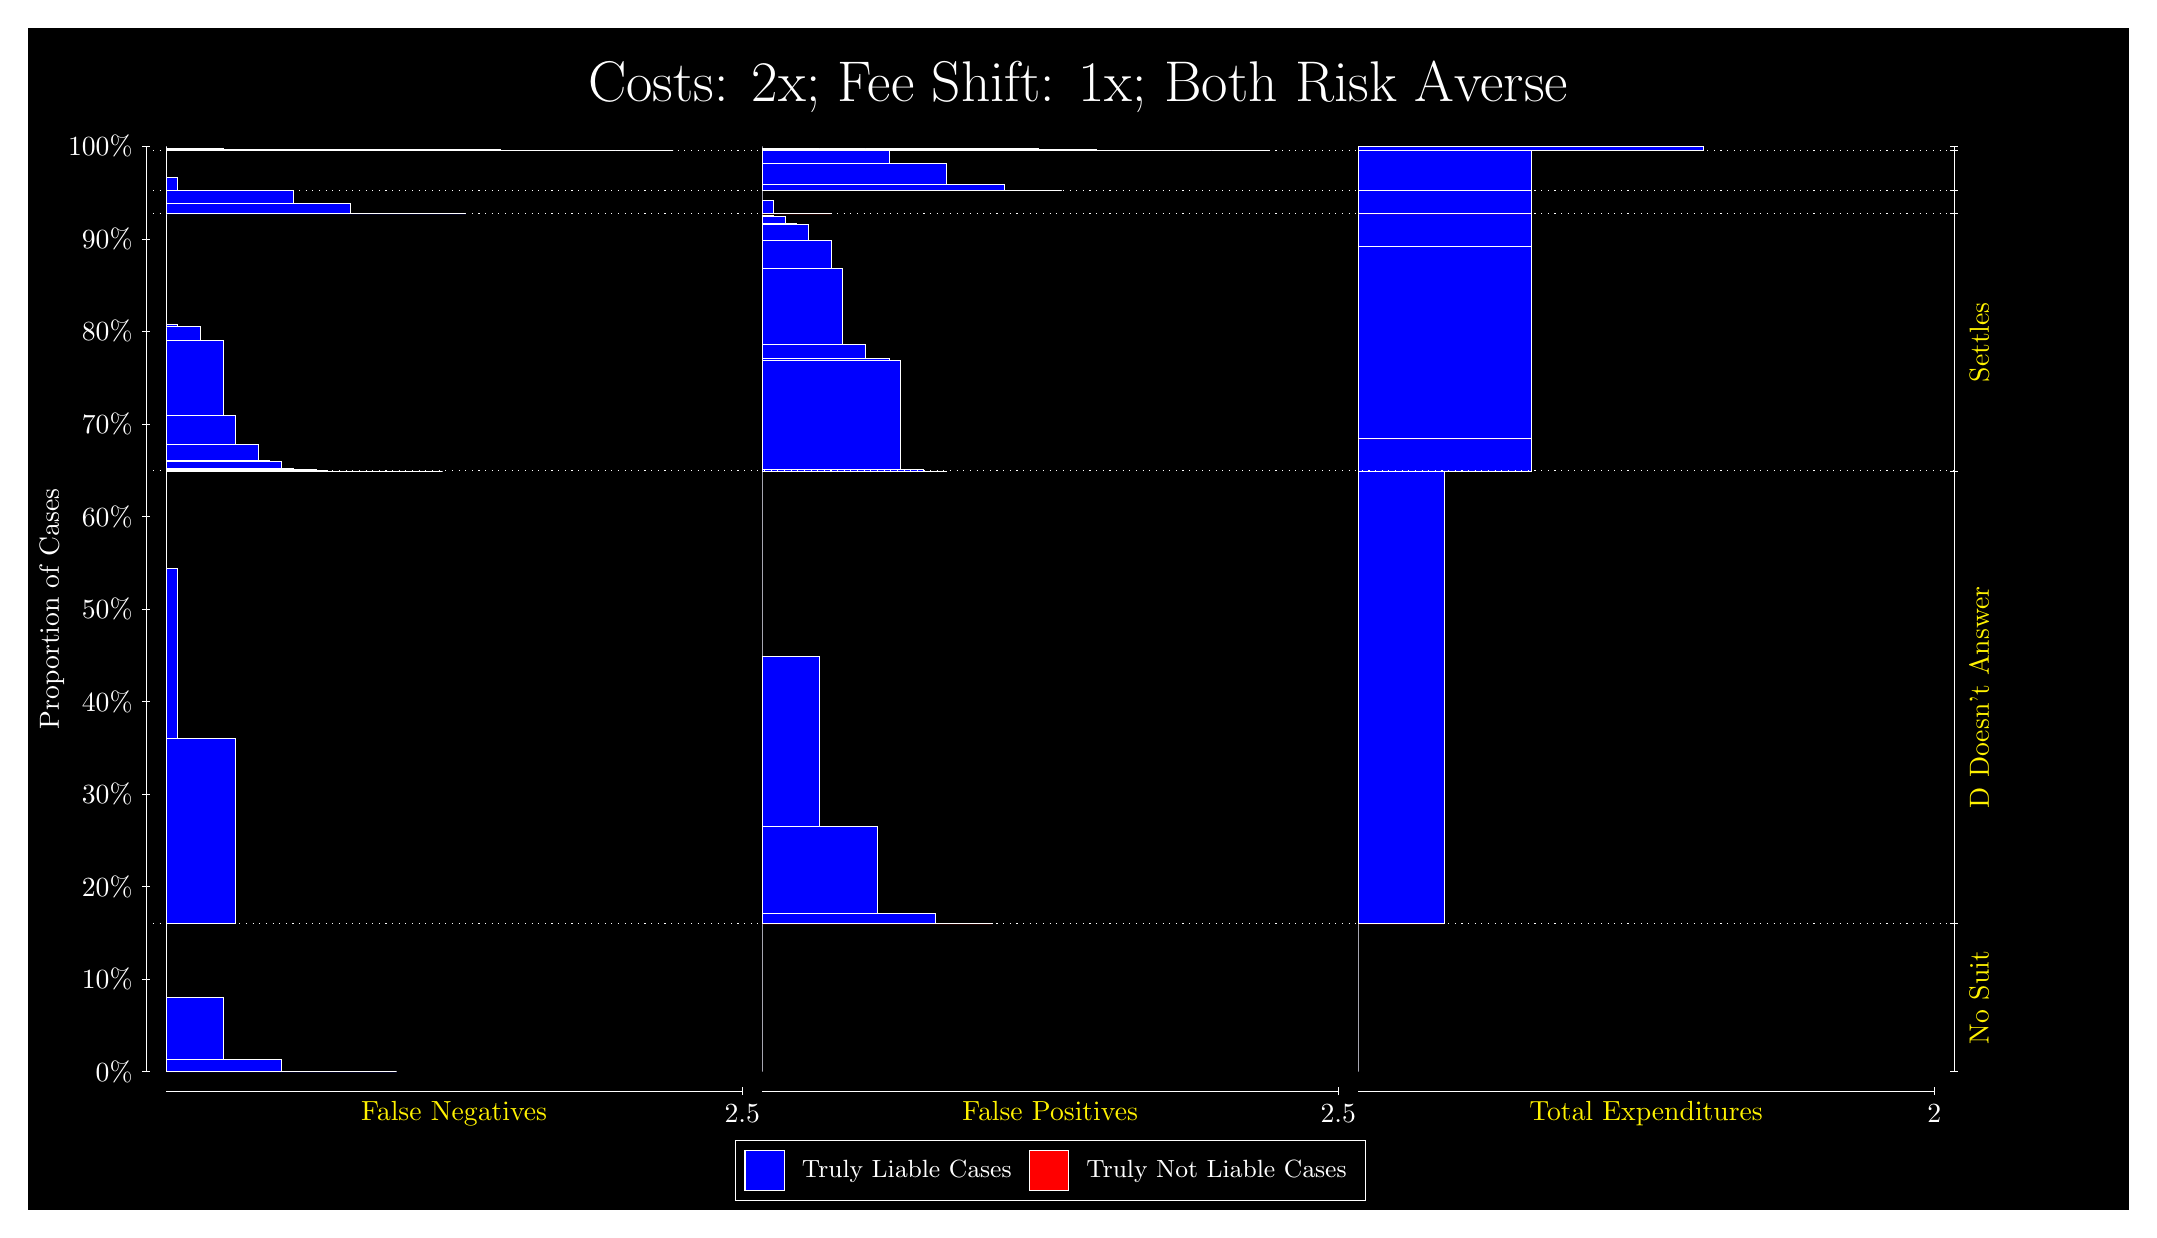
\begin{tikzpicture}
\draw[fill=black] (0,0) rectangle (26.667,15);
\draw[text=white] (0,13.5) rectangle (26.667,15) node[midway] {\huge Costs: 2x; Fee Shift: 1x; Both Risk Averse};
\draw[white, very thin] (1.5,1.75) -- (1.5,13.5);
\node[rotate=90, text=white, anchor=center] at (0.3, 7.625) {Proportion of Cases};
\draw[white, very thin] (1.45,1.75) -- (1.55,1.75);
\node[text=white, anchor=east] at (1.45, 1.75) {0\%};
\draw[white, very thin] (1.45,2.925) -- (1.55,2.925);
\node[text=white, anchor=east] at (1.45, 2.925) {10\%};
\draw[white, very thin] (1.45,4.1) -- (1.55,4.1);
\node[text=white, anchor=east] at (1.45, 4.1) {20\%};
\draw[white, very thin] (1.45,5.275) -- (1.55,5.275);
\node[text=white, anchor=east] at (1.45, 5.275) {30\%};
\draw[white, very thin] (1.45,6.45) -- (1.55,6.45);
\node[text=white, anchor=east] at (1.45, 6.45) {40\%};
\draw[white, very thin] (1.45,7.625) -- (1.55,7.625);
\node[text=white, anchor=east] at (1.45, 7.625) {50\%};
\draw[white, very thin] (1.45,8.8) -- (1.55,8.8);
\node[text=white, anchor=east] at (1.45, 8.8) {60\%};
\draw[white, very thin] (1.45,9.975) -- (1.55,9.975);
\node[text=white, anchor=east] at (1.45, 9.975) {70\%};
\draw[white, very thin] (1.45,11.15) -- (1.55,11.15);
\node[text=white, anchor=east] at (1.45, 11.15) {80\%};
\draw[white, very thin] (1.45,12.325) -- (1.55,12.325);
\node[text=white, anchor=east] at (1.45, 12.325) {90\%};
\draw[white, very thin] (1.45,13.5) -- (1.55,13.5);
\node[text=white, anchor=east] at (1.45, 13.5) {100\%};

\draw[white, very thin] (24.457,1.75) -- (24.457,13.5);
\draw[white, very thin] (24.407,1.75) -- (24.507,1.75);
\node[anchor=west] at (24.407, 1.75) {};
\draw[white, very thin] (24.407,3.6296) -- (24.507,3.6296);
\node[anchor=west] at (24.407, 3.6296) {};
\draw[white, very thin] (24.407,9.3775) -- (24.507,9.3775);
\node[anchor=west] at (24.407, 9.3775) {};
\draw[white, very thin] (24.407,12.646) -- (24.507,12.646);
\node[anchor=west] at (24.407, 12.646) {};
\draw[white, very thin] (24.407,12.942) -- (24.507,12.942);
\node[anchor=west] at (24.407, 12.942) {};
\draw[white, very thin] (24.407,13.449) -- (24.507,13.449);
\node[anchor=west] at (24.407, 13.449) {};
\draw[white, very thin] (24.407,13.5) -- (24.507,13.5);
\node[anchor=west] at (24.407, 13.5) {};

\draw[white, very thin, fill=blue] (1.75,1.75) rectangle (4.6775,1.75);
\draw[white, very thin, fill=blue] (1.75,1.75) rectangle (3.9457,1.7513);
\draw[white, very thin, fill=blue] (1.75,1.7513) rectangle (3.2138,1.9004);
\draw[white, very thin, fill=blue] (1.75,1.9004) rectangle (2.4819,2.6911);
\draw[white, very thin, fill=red] (1.75,2.6911) rectangle (1.75,2.6911);
\draw[white, very thin, fill=blue] (1.75,2.6911) rectangle (1.75,3.6296);
\draw[white, very thin, fill=blue] (1.75,3.6296) rectangle (2.6283,5.9776);
\draw[white, very thin, fill=blue] (1.75,5.9776) rectangle (1.8964,8.1383);
\draw[white, very thin, fill=red] (1.75,8.1383) rectangle (1.75,8.1383);
\draw[white, very thin, fill=blue] (1.75,8.1383) rectangle (1.75,9.3775);
\draw[white, very thin, fill=blue] (1.75,9.3775) rectangle (5.2631,9.3775);
\draw[white, very thin, fill=blue] (1.75,9.3775) rectangle (4.9703,9.3775);
\draw[white, very thin, fill=blue] (1.75,9.3775) rectangle (4.6775,9.3775);
\draw[white, very thin, fill=blue] (1.75,9.3775) rectangle (4.5312,9.3775);
\draw[white, very thin, fill=blue] (1.75,9.3775) rectangle (4.3848,9.3775);
\draw[white, very thin, fill=blue] (1.75,9.3775) rectangle (4.2384,9.3775);
\draw[white, very thin, fill=blue] (1.75,9.3775) rectangle (4.092,9.3775);
\draw[white, very thin, fill=blue] (1.75,9.3775) rectangle (3.9457,9.3789);
\draw[white, very thin, fill=blue] (1.75,9.3789) rectangle (3.7993,9.3868);
\draw[white, very thin, fill=blue] (1.75,9.3868) rectangle (3.6529,9.3935);
\draw[white, very thin, fill=blue] (1.75,9.3935) rectangle (3.5065,9.396);
\draw[white, very thin, fill=blue] (1.75,9.396) rectangle (3.3602,9.4148);
\draw[white, very thin, fill=blue] (1.75,9.4148) rectangle (3.2138,9.5026);
\draw[white, very thin, fill=blue] (1.75,9.5026) rectangle (3.0674,9.5128);
\draw[white, very thin, fill=blue] (1.75,9.5128) rectangle (2.921,9.713);
\draw[white, very thin, fill=blue] (1.75,9.713) rectangle (2.7746,9.7155);
\draw[white, very thin, fill=blue] (1.75,9.7155) rectangle (2.6283,10.078);
\draw[white, very thin, fill=blue] (1.75,10.078) rectangle (2.4819,11.034);
\draw[white, very thin, fill=blue] (1.75,11.034) rectangle (2.3355,11.034);
\draw[white, very thin, fill=blue] (1.75,11.034) rectangle (2.1891,11.211);
\draw[white, very thin, fill=blue] (1.75,11.211) rectangle (2.0428,11.211);
\draw[white, very thin, fill=blue] (1.75,11.211) rectangle (1.8964,11.239);
\draw[white, very thin, fill=red] (1.75,11.239) rectangle (1.75,11.239);
\draw[white, very thin, fill=blue] (1.75,11.239) rectangle (1.75,12.646);
\draw[white, very thin, fill=blue] (1.75,12.646) rectangle (5.5558,12.646);
\draw[white, very thin, fill=blue] (1.75,12.646) rectangle (4.8239,12.647);
\draw[white, very thin, fill=blue] (1.75,12.647) rectangle (4.092,12.773);
\draw[white, very thin, fill=blue] (1.75,12.773) rectangle (3.3602,12.939);
\draw[white, very thin, fill=blue] (1.75,12.939) rectangle (2.6283,12.942);
\draw[white, very thin, fill=red] (1.75,12.942) rectangle (1.75,12.942);
\draw[white, very thin, fill=blue] (1.75,12.942) rectangle (2.6283,12.943);
\draw[white, very thin, fill=blue] (1.75,12.943) rectangle (1.8964,13.103);
\draw[white, very thin, fill=red] (1.75,13.103) rectangle (1.75,13.103);
\draw[white, very thin, fill=blue] (1.75,13.103) rectangle (1.75,13.449);
\draw[white, very thin, fill=blue] (1.75,13.449) rectangle (8.1906,13.449);
\draw[white, very thin, fill=blue] (1.75,13.449) rectangle (7.4587,13.449);
\draw[white, very thin, fill=blue] (1.75,13.449) rectangle (6.7268,13.449);
\draw[white, very thin, fill=blue] (1.75,13.449) rectangle (5.9949,13.457);
\draw[white, very thin, fill=blue] (1.75,13.457) rectangle (5.2631,13.467);
\draw[white, very thin, fill=blue] (1.75,13.467) rectangle (4.5312,13.468);
\draw[white, very thin, fill=blue] (1.75,13.468) rectangle (3.9457,13.468);
\draw[white, very thin, fill=blue] (1.75,13.468) rectangle (3.7993,13.468);
\draw[white, very thin, fill=blue] (1.75,13.468) rectangle (3.2138,13.468);
\draw[white, very thin, fill=blue] (1.75,13.468) rectangle (2.4819,13.472);
\draw[white, very thin, fill=red] (1.75,13.472) rectangle (1.75,13.472);
\draw[white, very thin, fill=blue] (1.75,13.472) rectangle (1.75,13.5);
\draw[white, very thin, fill=red] (9.3189,1.75) rectangle (9.3189,1.75);
\draw[white, very thin, fill=blue] (9.3189,1.75) rectangle (9.3189,3.6296);
\draw[white, very thin, fill=red] (9.3189,3.6296) rectangle (12.246,3.6296);
\draw[white, very thin, fill=blue] (9.3189,3.6296) rectangle (12.246,3.6308);
\draw[white, very thin, fill=blue] (9.3189,3.6308) rectangle (11.515,3.7625);
\draw[white, very thin, fill=blue] (9.3189,3.7625) rectangle (10.783,4.8688);
\draw[white, very thin, fill=blue] (9.3189,4.8688) rectangle (10.051,7.0295);
\draw[white, very thin, fill=blue] (9.3189,7.0295) rectangle (9.3189,9.3775);
\draw[white, very thin, fill=red] (9.3189,9.3775) rectangle (11.661,9.3775);
\draw[white, very thin, fill=blue] (9.3189,9.3775) rectangle (11.661,9.3776);
\draw[white, very thin, fill=red] (9.3189,9.3776) rectangle (11.368,9.3776);
\draw[white, very thin, fill=blue] (9.3189,9.3776) rectangle (11.368,9.4048);
\draw[white, very thin, fill=red] (9.3189,9.4048) rectangle (11.075,9.4048);
\draw[white, very thin, fill=blue] (9.3189,9.4048) rectangle (11.075,10.785);
\draw[white, very thin, fill=blue] (9.3189,10.785) rectangle (10.929,10.813);
\draw[white, very thin, fill=red] (9.3189,10.813) rectangle (10.783,10.813);
\draw[white, very thin, fill=blue] (9.3189,10.813) rectangle (10.783,10.813);
\draw[white, very thin, fill=blue] (9.3189,10.813) rectangle (10.636,10.99);
\draw[white, very thin, fill=red] (9.3189,10.99) rectangle (10.49,10.99);
\draw[white, very thin, fill=blue] (9.3189,10.99) rectangle (10.49,10.99);
\draw[white, very thin, fill=blue] (9.3189,10.99) rectangle (10.344,11.946);
\draw[white, very thin, fill=blue] (9.3189,11.946) rectangle (10.197,12.309);
\draw[white, very thin, fill=blue] (9.3189,12.309) rectangle (10.051,12.311);
\draw[white, very thin, fill=blue] (9.3189,12.311) rectangle (9.9044,12.511);
\draw[white, very thin, fill=blue] (9.3189,12.511) rectangle (9.758,12.521);
\draw[white, very thin, fill=blue] (9.3189,12.521) rectangle (9.6116,12.609);
\draw[white, very thin, fill=blue] (9.3189,12.609) rectangle (9.4652,12.628);
\draw[white, very thin, fill=blue] (9.3189,12.628) rectangle (9.3189,12.646);
\draw[white, very thin, fill=red] (9.3189,12.646) rectangle (10.197,12.646);
\draw[white, very thin, fill=blue] (9.3189,12.646) rectangle (10.197,12.649);
\draw[white, very thin, fill=blue] (9.3189,12.649) rectangle (9.4652,12.815);
\draw[white, very thin, fill=blue] (9.3189,12.815) rectangle (9.3189,12.942);
\draw[white, very thin, fill=red] (9.3189,12.942) rectangle (13.125,12.942);
\draw[white, very thin, fill=blue] (9.3189,12.942) rectangle (13.125,12.942);
\draw[white, very thin, fill=blue] (9.3189,12.942) rectangle (12.393,13.015);
\draw[white, very thin, fill=blue] (9.3189,13.015) rectangle (11.661,13.287);
\draw[white, very thin, fill=blue] (9.3189,13.287) rectangle (10.929,13.447);
\draw[white, very thin, fill=blue] (9.3189,13.447) rectangle (10.197,13.449);
\draw[white, very thin, fill=red] (9.3189,13.449) rectangle (15.759,13.449);
\draw[white, very thin, fill=blue] (9.3189,13.449) rectangle (15.759,13.449);
\draw[white, very thin, fill=blue] (9.3189,13.449) rectangle (15.028,13.449);
\draw[white, very thin, fill=red] (9.3189,13.449) rectangle (15.028,13.449);
\draw[white, very thin, fill=blue] (9.3189,13.449) rectangle (15.028,13.449);
\draw[white, very thin, fill=blue] (9.3189,13.449) rectangle (14.296,13.449);
\draw[white, very thin, fill=red] (9.3189,13.449) rectangle (14.296,13.449);
\draw[white, very thin, fill=blue] (9.3189,13.449) rectangle (14.296,13.45);
\draw[white, very thin, fill=blue] (9.3189,13.45) rectangle (13.564,13.45);
\draw[white, very thin, fill=red] (9.3189,13.45) rectangle (13.564,13.45);
\draw[white, very thin, fill=blue] (9.3189,13.45) rectangle (13.564,13.461);
\draw[white, very thin, fill=blue] (9.3189,13.461) rectangle (12.832,13.461);
\draw[white, very thin, fill=blue] (9.3189,13.461) rectangle (12.832,13.476);
\draw[white, very thin, fill=blue] (9.3189,13.476) rectangle (12.1,13.481);
\draw[white, very thin, fill=blue] (9.3189,13.481) rectangle (11.368,13.481);
\draw[white, very thin, fill=red] (9.3189,13.481) rectangle (10.783,13.481);
\draw[white, very thin, fill=blue] (9.3189,13.481) rectangle (10.783,13.481);
\draw[white, very thin, fill=blue] (9.3189,13.481) rectangle (10.636,13.481);
\draw[white, very thin, fill=red] (9.3189,13.481) rectangle (10.051,13.481);
\draw[white, very thin, fill=blue] (9.3189,13.481) rectangle (10.051,13.481);
\draw[white, very thin, fill=red] (9.3189,13.481) rectangle (9.3189,13.481);
\draw[white, very thin, fill=blue] (9.3189,13.481) rectangle (9.3189,13.5);
\draw[white, very thin, fill=red] (16.888,1.75) rectangle (16.888,1.75);
\draw[white, very thin, fill=blue] (16.888,1.75) rectangle (16.888,3.6296);
\draw[white, very thin, fill=red] (16.888,3.6296) rectangle (17.986,3.6296);
\draw[white, very thin, fill=blue] (16.888,3.6296) rectangle (17.986,9.3775);
\draw[white, very thin, fill=red] (16.888,9.3775) rectangle (19.083,9.3775);
\draw[white, very thin, fill=blue] (16.888,9.3775) rectangle (19.083,9.7881);
\draw[white, very thin, fill=red] (16.888,9.7881) rectangle (19.083,9.7881);
\draw[white, very thin, fill=blue] (16.888,9.7881) rectangle (19.083,12.236);
\draw[white, very thin, fill=red] (16.888,12.236) rectangle (19.083,12.236);
\draw[white, very thin, fill=blue] (16.888,12.236) rectangle (19.083,12.646);
\draw[white, very thin, fill=red] (16.888,12.646) rectangle (19.083,12.646);
\draw[white, very thin, fill=blue] (16.888,12.646) rectangle (19.083,12.942);
\draw[white, very thin, fill=red] (16.888,12.942) rectangle (19.083,12.942);
\draw[white, very thin, fill=blue] (16.888,12.942) rectangle (19.083,13.449);
\draw[white, very thin, fill=red] (16.888,13.449) rectangle (21.279,13.449);
\draw[white, very thin, fill=blue] (16.888,13.449) rectangle (21.279,13.45);
\draw[white, very thin, fill=red] (16.888,13.45) rectangle (21.279,13.45);
\draw[white, very thin, fill=blue] (16.888,13.45) rectangle (21.279,13.5);
\draw[white, dotted] (1.5,3.6296) -- (24.457,3.6296);
\draw[white, dotted] (1.5,9.3775) -- (24.457,9.3775);
\draw[white, dotted] (1.5,12.646) -- (24.457,12.646);
\draw[white, dotted] (1.5,12.942) -- (24.457,12.942);
\draw[white, dotted] (1.5,13.449) -- (24.457,13.449);
\draw[white, very thin] (1.75,1.5) -- (9.0689,1.5);
\node[text=yellow, anchor=north] at (5.4094, 1.5) {False Negatives};
\draw[white, very thin] (9.0689,1.45) -- (9.0689,1.55);
\node[text=white, anchor=north] at (9.0689, 1.45) {2.5};

\draw[white, very thin] (9.3189,1.5) -- (16.638,1.5);
\node[text=yellow, anchor=north] at (12.978, 1.5) {False Positives};
\draw[white, very thin] (16.638,1.45) -- (16.638,1.55);
\node[text=white, anchor=north] at (16.638, 1.45) {2.5};

\draw[white, very thin] (16.888,1.5) -- (24.207,1.5);
\node[text=yellow, anchor=north] at (20.547, 1.5) {Total Expenditures};
\draw[white, very thin] (24.207,1.45) -- (24.207,1.55);
\node[text=white, anchor=north] at (24.207, 1.45) {2};

\node[text=yellow, centered, rotate=90] at (24.777, 2.6898) {No Suit};
\node[text=yellow, centered, rotate=90] at (24.777, 6.5036) {D Doesn't Answer};
\node[text=yellow, centered, rotate=90] at (24.777, 11.012) {Settles};




\draw (12.978300999999998,1.5) node[draw=none] (baseCoordinate) {};
\begin{scope}[align=center]
        \matrix[scale=0.5, draw=white, below=0.5cm of baseCoordinate, nodes={draw}, column sep=0.1cm]{
            \node[rectangle, draw, minimum width=0.5cm, minimum height=0.5cm, fill=blue] {}; &
            \node[draw=none, font=\small, text=white] (B) {Truly Liable Cases}; &
            \node[rectangle, draw, minimum width=0.5cm, minimum height=0.5cm, fill=red] {}; &
            \node[draw=none, font=\small, text=white] (B) {Truly Not Liable Cases}; \\
            };
\end{scope}

\end{tikzpicture}
\end{document}